\chapter{Résultats}
\section{Préambule}
\subsection{Description de la machine physique }
La machine mis à disposition est un serveur avec pour Stockage de masse quatre disque dur de 1TB chacun mis en RAID 0. Voici en détails les caractéristiques :


  PROCESSOR:          2 x Intel Xeon L5630 @ 2.13GHz (16 Cores)\newline
    Core Count:       4\newline
    Thread Count:     16\newline
    Extensions:       SSE 4.2\newline
    Cache Size:       12288 KB\newline
    Microcode:        0x13\newline

  GRAPHICS:           Matrox s MGA G200eW WPCM450\newline
    Screen:           1280x1024\newline

  MOTHERBOARD:        Dell 0MD99X\newline
    Memory:           18 x 16384 MB DDR3-1333MHz\newline
    Chipset:          Intel 5520 I/O + ICH9\newline
    Network:          Broadcom NetXtreme II BCM5709 Gigabit\newline

  DISK:               3999GB Virtual Disk\newline
    File-System:      ext4\newline
    Mount Options:    data=ordered errors=remount-ro relatime rw\newline
    Disk Scheduler:   CFQ\newline

  OPERATING SYSTEM:   Debian 8.7\newline
    Kernel:           3.16.0-4-amd64 (x86\_64)\newline
    Compiler:         GCC 4.9.2\newline

\subsection{Sur les machines virtuelles}
Lors des tests l'ensemble des postulats sur le versionnage des système d'exploitation et autres caractéristiques possiblement mouvante sont statique, et son donc respecte.
Un détails qui n'as pas été préciser lors du rapport auparavant. Le nombre de machine active durant les tests sont égales aux nombre de machine qui effectue les tests. Il n'y a aucun moment, ou le nombre de machine allume est supérieur a ceux des machines en cours d’évaluations.
De plus les machines virtuelles produite par KVM et QEMU sont dote d'un disque qcow2 et utilisant virtio.
\newpage
\section{Partie Processeurs}
\begin{figure}[h]
   \begin{minipage}[c]{.46\linewidth}
	   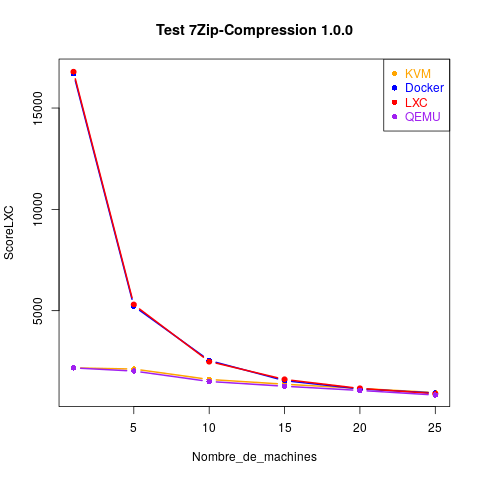
\includegraphics[scale=0.55]{resultats/7zip.png}
   \end{minipage} \hfill
   \begin{minipage}[c]{.46\linewidth}
   	 Comme expliquer auparavant, il s'agit d'un test de 7-Zip avec p7zip. Le premier test exécute sur les machines. Le test est de type : Plus haut le score est, meilleur c'est.  On observe assez rapidement que en mono-machine, la technologies des conteneurs est cohérente entre elles LXC, Docker sont très clairement meilleurs. Par contre le nombre de machines augmentant,  les scores se resserrent vers ceux de KVM et QEMU. On peut conjecturer que KVM et QEMU serait plus stables avec un nombre de machines qui augmente. On remarque que les technologies de conteneurisation sont proches des meilleurs résultats obtenus sur la machines physique. 
   	 \end{minipage}
\end{figure}
\begin{figure}[h]
   \begin{minipage}[c]{.46\linewidth}
	  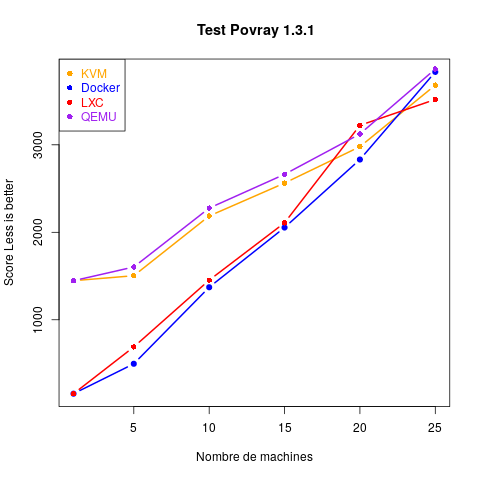
\includegraphics[scale=0.55]{resultats/povray.png}
   \end{minipage} \hfill
   \begin{minipage}[c]{.46\linewidth}
   	  Il s'agit d'un test de POV-Ray, The Persistence of Vision Raytracer. POV-Ray est utilisé pour créer des graphiques 3D à l'aide de ray-tracing. On remarque que KVM et QEMU sont encore une fois assez proche c'est d'autant plus notable que le score est précis et se différencie d'une moyenne de 100-200 d’écart ! Ceci dit, on pourrait interpreter les courbes de KVM et QEMU, quasiment proche d'une courbe lineaire, cette conjecture pourrait etrte confirmer si les tests avait ete fait avec un pas de un par un pour le nombre de machines. 
      On remarque encore une fois que les technologies de conteneurisation sont proches des meilleurs résultats obtenus sur la machines physique
   \end{minipage}
\end{figure}

\newpage
\begin{figure}[h]
   \begin{minipage}[c]{.46\linewidth}
	 Il s'agit d'un test de performance de Crafty, un moteur d'échecs open source avancé. Ici c'est le temps qui est contrôle, et donc assez logiquement moindre il est  meilleur cela en est. Assez logiquement le profile de la courbe est proche d'une courbe linéaire.
	  On remarque que les technologies de virtualisation sont proches des meilleurs résultats obtenus sur la machines physique, cette fois ci les conteneurs sont assez proches des hyperviseurs classique. 
   \end{minipage} \hfill
   \begin{minipage}[c]{.46\linewidth}
   	  
   	  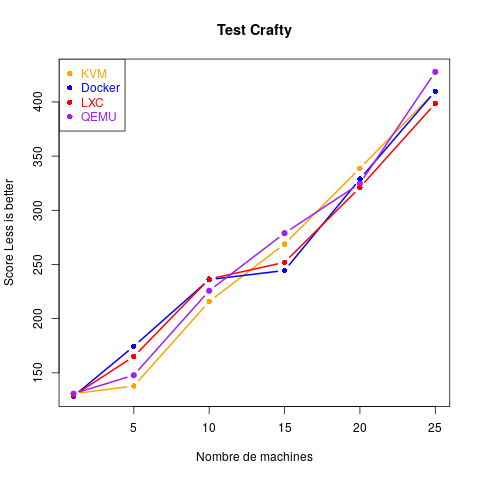
\includegraphics[scale=0.55]{resultats/Crafty.png}
   \end{minipage}
\end{figure}
\begin{figure}[h]
   \begin{minipage}[c]{.46\linewidth}
	 Il s'agit d'un test de performance du TSCP, le programme Simple Chess de Tom Kerrigan. Cette fois ci un autre profile de test, celui du plus haut le score, mieux c'est. Docker se dégage presque comme une courbe linéaire descendante. Contrairement aux autres technologies qui semble perdre enormement de performance au delà de 10 machines. Cependant pour 20 machines, LXC et KVM on des scores légèrement meilleur que sur 15 machines, il se peut que ces chiffres soit non pas biaise mais que par le biais de changement de contexte au niveau processeur, une meilleur moyenne en est dégager. Il faut aussi rappeler que les scores afficher sont des moyenne des scores obtenue sur les n machines. De plus, ces chiffres avait eux même une intervalle de confiance de 2.5\% a 5\% . Donc il n'y a rien de bien grave le profil révélé n'est pas assez distinct .
   \end{minipage} \hfill
   \begin{minipage}[c]{.46\linewidth}
   	  
       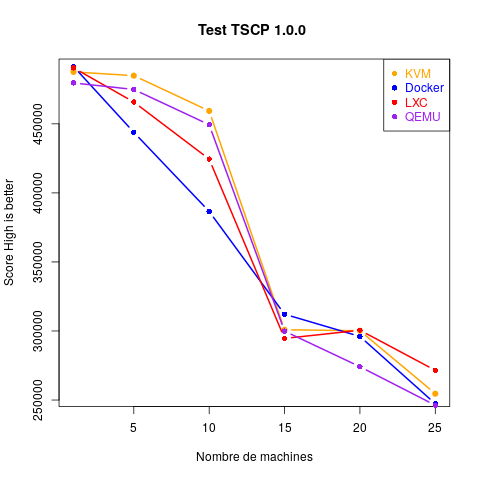
\includegraphics[scale=0.55]{resultats/TSCP.png}
   \end{minipage}
\end{figure}



\newpage
\section{Partie Disque dur }
\begin{figure}[!h]
\centering
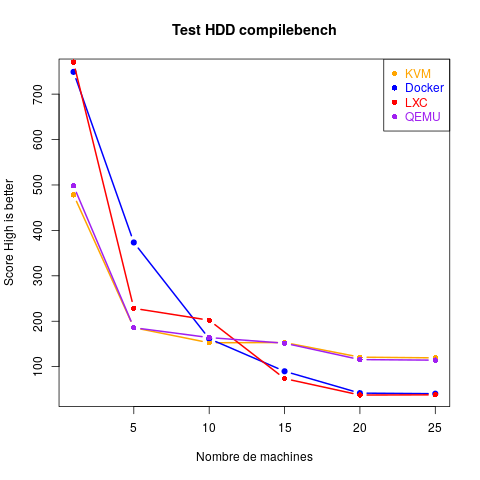
\includegraphics[scale=0.8]{resultats/compilebench.png}
\end{figure}
Compilebench essaie de "stresse" un système de fichiers en simulant une partie de l'IO du disque commun dans la création, la compilation, l'affichage et la lecture d'un noyau linux . Il mesure indirectement la façon dont les systèmes de fichiers peuvent maintenir la localisation du répertoire lorsque le disque se remplit et l'âge des répertoires. Ce test actuel est configuré pour utiliser le mode makej avec 10 répertoires initiaux. Ici, encore une fois, plus le score est haut mieux c'est.
Ici il y a un réel tendance, les hyperviseurs KVM et QEMU sont vraiment meilleurs quand le nombre machines augmente. LXC marquait une différence net avec Docker sur 5 et 10 machines mais il se resserre pour être extrêmement proche .
Malgré tout, Docker, LXC sont proche des résultats obtenu par la machines physique.
\newpage
\section{Partie Mémoire}
\begin{figure}[h]
   \begin{minipage}[c]{.46\linewidth}
	   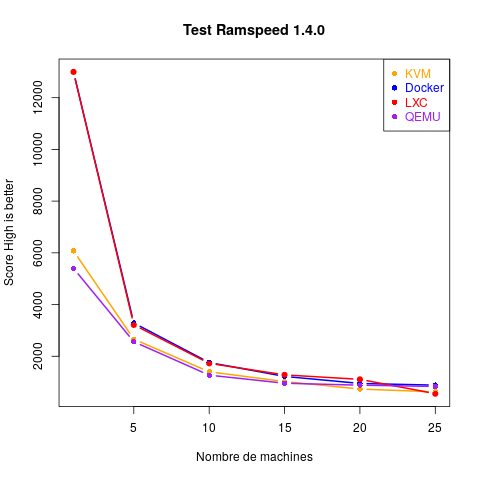
\includegraphics[scale=0.5]{resultats/ramspeed.png}
   \end{minipage} \hfill
   \begin{minipage}[c]{.46\linewidth}
     Ce test, teste la performance de la mémoire système (RAM).C'est un test cherchant le meilleur par le meilleur score. Encore une fois une conjecture émise plus haut se distingue réellement, les conteneurs on une performance très proche de la machines physique au début ( C'est a dire quand il n'y a que une machine active) L’écrasement de ce test est assez vite amène et les technologie se retrouvent être dans le même écart. D'autant plus que les résultat a 100 près alors que le score de la machines physique est de plus de 12000 .
   \end{minipage}
\end{figure}

\begin{figure}[h]
   \begin{minipage}[c]{.46\linewidth}
	 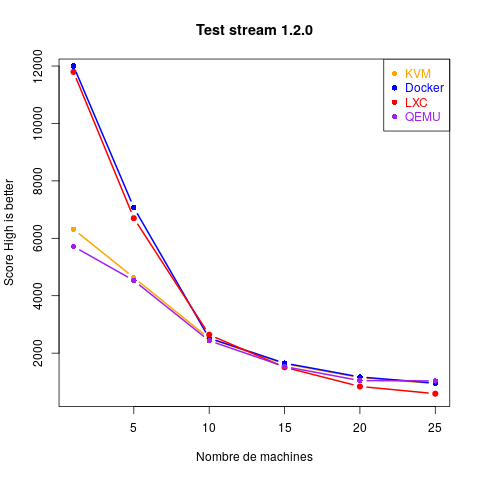
\includegraphics[scale=0.5]{resultats/stream.png}
   \end{minipage} \hfill
   \begin{minipage}[c]{.46\linewidth}
     Ce test, teste la performance de la mémoire système (RAM).C'est un test cherchant le meilleur par le meilleur score. Encore une fois une conjecture émise plus haut se distingue réellement, comme dans le graphique précédent, on arrive on même conclusion.
   \end{minipage}
\end{figure}
\newpage
\begin{figure}[h]
\centering
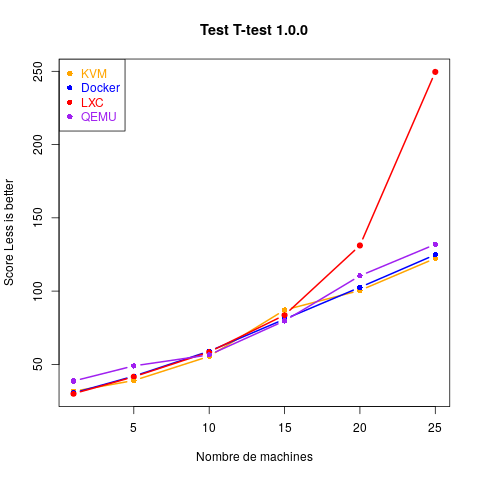
\includegraphics[scale=0.8]{resultats/t-test.png} 
\end{figure}
Il s'agit d'un test de t-test1 pour les benchmarks d'allocateur de mémoire de base. Notez que ce profil de test est actuellement très basique et que le temps global inclut le temps de preparation de la compilation t-test1. La politique du moins bon score est le meilleur sur ce test.
Ainsi quelque chose d'assez clair c'est que a part pour LXC, les courbes sont assez linéaire. Pour LXC, on aurait presque tendance a dire que elle a une allure exponentielle .
\newpage
\section{Partie Réseaux }
\begin{figure}[h]
\centering
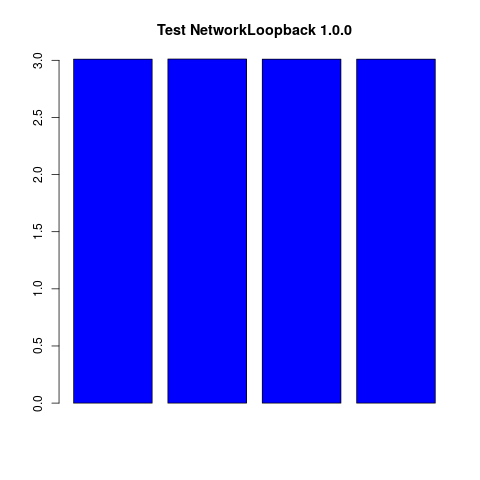
\includegraphics[scale=0.8]{resultats/netloop.png}
\end{figure}
Ce test mesure les performances de la loopback à l'aide d'un micro-benchmark pour mesurer les performances TCP.
Il en est ressortie que quelquesoit le nombre de machines active. La performance reste identique pour quelquesoit la technologie de virtualisation utilise. Ici meme si le resultat affiche est petit, et identique. Ce test se base sur une comparaison de LIB, encore une du plus petit est le meilleur.
\newpage
\section{Partie Web}
\begin{figure}[h]
   \begin{minipage}[c]{.46\linewidth}
	   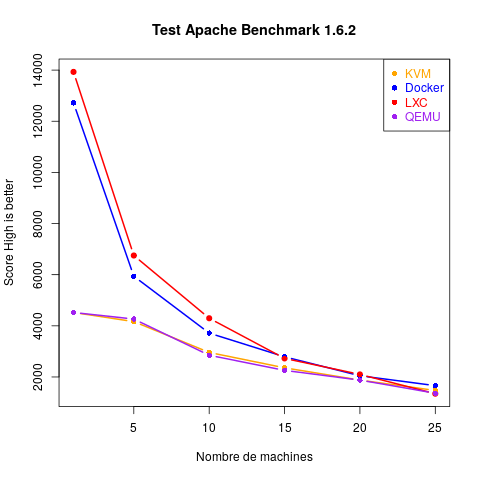
\includegraphics[scale=0.5]{resultats/apache.png}
   \end{minipage} \hfill
   \begin{minipage}[c]{.46\linewidth}
      	Il s'agit d'un test d'ab, qui est le programme de référence Apache. Ce profil de test mesure le nombre de demandes par seconde qu'un système donné peut supporter lors de la réalisation de 1 000 000 de demandes avec 100 requêtes effectuées simultanément. Évidemment plus le système meilleur le résultat seras.Malgré tout, Docker, LXC sont proche des résultats obtenu par la machines physique.Il y a manifestement un goulot d’étranglement qui opère des les 10 machines actives.
   \end{minipage}
\end{figure}

\begin{figure}[h]
   \begin{minipage}[c]{.46\linewidth}
	   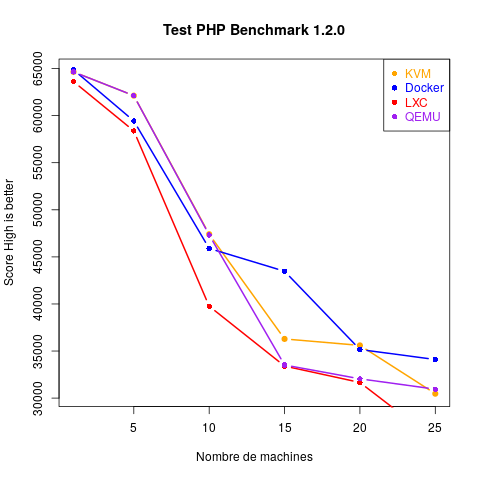
\includegraphics[scale=0.5]{resultats/phpbench.png}
   \end{minipage} \hfill
   \begin{minipage}[c]{.46\linewidth}
      	PHPBench est une suite de référence pour PHP. Il effectue un grand nombre de tests simples afin de classer divers aspects de l'interpréteur PHP. PHPBench peut être utilisé pour comparer le matériel, les systèmes d'exploitation, les versions PHP, les accélérateurs PHP et les caches, les options de compilation, etc. Le nombre d'itérations utilisées est de 1 000 000.
Évidemment plus le système meilleur le résultat seras.Malgré tout les différentes technologie de virtualisation sont proche des résultats obtenu par la machine physique.Il y a manifestement un goulot d’étranglement qui opère des les 10 machines actives.
   \end{minipage}
\end{figure}